\section{Real-Time Control System and Hardware Platform}
\label{sec:ch2:hw}

\begin{figure*}[t]
\centering
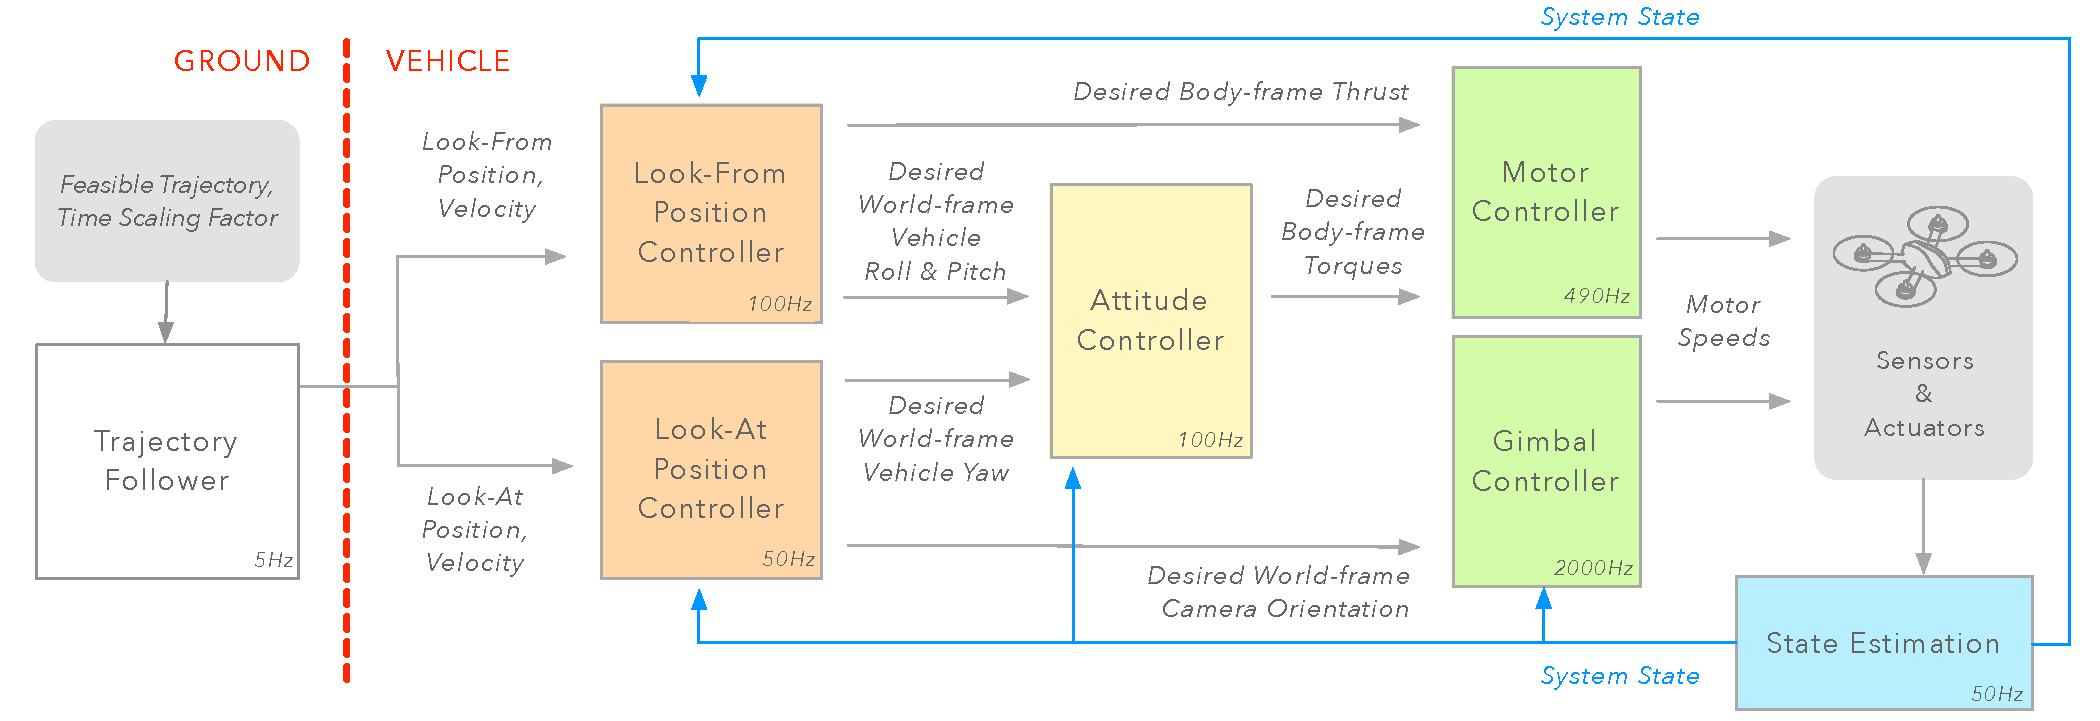
\includegraphics[width=6.0in]{images/2015_siggraph_asia/ControlAlgorithm}
\caption{
Block diagram of our real-time control system for executing camera trajectories.
On a ground station (left), our trajectory follower (white) samples the camera trajectory, transmitting the sampled position and velocity of look-at and look-from points to the quadrotor.
Our trajectory follower allows the user to optionally adjust a time scaling factor, to execute the trajectory faster or slower.
On board the quadrotor (right), the higher-level look-from and look-at position controllers interface with a lower-level attitude controller (yellow) and motor controller (green), similar to those described by Kumar and Michael~\protect\shortcite{kumar:2012}.
}
\label{fig:ch2:controlsystem}
\end{figure*}

In this section, we describe the real-time control system and hardware platform we use to execute camera trajectories autonomously and capture real video footage.
%At a high level, we use the camera trajectory computed in Section~\ref{section:synthesizing_virtual_camera_trajectories} to drive a feedback controller running on a real-world quadrotor.
%This feedback controller compensates for unexpected disturbances, unmodeled forces, and sensor noise, without having to recompute the camera trajectory.

\paragraph{Real-Time Control System}
We show a block diagram of our real-time control system in Figure~\ref{fig:ch2:controlsystem}.
We build our real-time control system on top of the open source \textsc{ArduPilot} autopilot software \cite{apm:2015}. 
The \textsc{ArduPilot} software runs on board the quadrotor, and provides a hierarchical feedback controller for following camera trajectories, similar to the controller described by Kumar and Michael~\shortcite{kumar:2012}. 
The \textsc{ArduPilot} feedback controller takes as input the position and velocity of look-at and look-from points along a camera trajectory.
Our real-time control system runs on a ground station.
Our system executes the user's intended camera trajectory by sampling the position and velocity of look-at and look-from points along the trajectory, and transmitting these quantities to the quadrotor.

%We use a camera trajectory computed in Section~\ref{section:synthesizing_virtual_camera_trajectories} to drive a feedback controller running on a real-world quadrotor.
%This feedback controller compensates for unexpected disturbances, unmodeled forces, and sensor noise, without having to recompute the camera trajectory.
%This feedback controller takes as input the position and velocity of look-at and look-from points along the intended camera trajectory.

%We use this controller to actuate the desired kinematic behavior of the look-at and look-from points. 
%We start by taking a time sample of the user's trajectory. 
%The resulting positions and velocities are transmitted to the quadrotor during flight. 
%Onboard, our look-from controller calculates the desired quadrotor orientation and thrust to follow the look-from point given the current vehicle state.  
%Our look-at position controller calculates the desired camera orientation and vehicle yaw to follow the look-at point given the current vehicle position. 
%The outputs from the look-from and look-at controllers are actuated by the attitude, gimbal and motor controllers provided in ArduPilot.

\paragraph{Time Scaling and Safety}
While the camera trajectory is being executed, our real-time control system allows the user to optionally adjust a time scaling factor.
By default, our system samples the camera trajectory uniformly in time.
If the user adjusts the time scaling factor, our system applies a linear scaling to the time step used to determine the next sampling location along the trajectory.
Using our time scaling functionality, we implement a \emph{full stop} command, which is an important safety feature.
Setting the time scaling factor to 0 pauses the quadrotor at its current position.
This allows the user to abort capture at any time, and helps to avoid crashes.

%The other kinematic quantities are scaled appropriately as well. 
%Using this approach, we implement a useful safety feature in the form of a ``full stop'' command. A time scaling factor of zero pauses the desired position with a velocity of zero at the current point on the trajectory. This allows the user to abort capture at any moment, and helps to avoid crashes.

% This quadrotor runs the open source ArduPilot software~\cite{apm:2015}
% on its onboard Pixhawk autopilot computer~\cite{meier2012pixhawk}.
% This codebase exposes a set of commands using the MAVLink
% protocol~\cite{mavlink:2015} that can be triggered from a gound station computer over the telemetry radio link. Horus streams the trajectory as a sequence of POSVEL and SET\_ROI commands. This provides the desired setpoints for the onboard PID-based feedback controller to move to the quadrotor along the look-from trajectory and point the camera at the look-at trajectory. 

\paragraph{Hardware Platform}
Our hardware platform consists of an \textsc{3D Robotics IRIS+} quadrotor~\cite{3dr_iris_p:2014} running the open source \textsc{ArduPilot} autopilot software~\cite{apm:2015} on a \textsc{Pixhawk} autopilot computer~\cite{meier:2012}.
%We attached a remote camera view to aid rapid iteration and visual shot design.
We equip our quadrotor with a 2-axis gimbal and a \textsc{GoPro Hero 4 Black} camera.
At the time of publication, this hardware setup is priced at \$1300, and is representative of an entry-level quadrotor for aerial cinematography.  

\paragraph{System Identification}
We determined the system parameters used in our quadrotor camera model, which are specific to our hardware, partially through direct measurement and partially through published engineering specifications.
We used a dynamometer to measure the maximum force and torque our rotors could generate, and estimated the moment of inertia from the quadrotor's mass and shape.
We used the maximum lean angles, maximum velocities, and maximum accelerations published by the \textsc{ArduPilot} community~\cite{apm:2015}. 

%\paragraph{Accuracy}
%The accuracy of our system is limited by the on-board state estimation of our quadrotor hardware.
%The \textsc{IRIS+} is equiped with a standard GPS receiver, a barometer, and an inertial measurement unit (IMU) consisting of a gyroscope, an accelerometer, and a magnetometer. 
%The quadrotor's positioning accuracy depends on the on-board GPS sensor and barometer.
%Horizontal positioning is generally accurate to within 2.8m~\cite{kaplan:2006}.
%In our experience, vertical positioning is generally accurate to within 2.0m.
%GPS-based velocity measurements are generally accurate to within 0.1m/s~\cite{ublox:2013}.

%Although more accurate on-board state estimation will surely enable more challenging shots, we found in Section \ref{results} that our users could successfully produce a wide variety of compelling shots using this hardware.

%Altimiter accuracy and precision suffer from local atmospheric effects.
%In informal bench testing we've found the altimeter's altitude estimate drifts in excess of 2 meters over 30 minutes.
%Although higher accuracies will enable more challenging shots (e.g. close-ups that require very precise positioning), we find in section ~\ref{results} that our users can produce a wide variety of interesting shots using this hardware.
